\documentclass[12pt]{article}
\usepackage[utf8]{inputenc}
\usepackage{amsmath,amssymb}
\usepackage{unicode-math}
\usepackage[T2A]{fontenc}
\usepackage[russian]{babel}
\usepackage{graphicx}
\usepackage{subfigure}
\usepackage{subcaption}
\usepackage{url}
\usepackage{float}


\DeclareGraphicsExtensions{.pdf,.png,.jpg}
\usepackage{hyperref}
\usepackage{wrapfig}
\usepackage[left=20mm, top=20mm, right=10mm, bottom=20mm]{geometry}

\usepackage{amsmath} 
\usepackage{amsfonts} 
\usepackage{amssymb} 
\usepackage{wasysym} 
\usepackage{fancyhdr}

\pagestyle{fancy}
\fancyhf{}
\lhead{Семинар 6. Уровни энергии в различных системах}
\rhead{\textit{Клименок К.Л., МФТИ 2020}}
\rfoot{\thepage}



\begin{document} 
\title{\textbf{Семинар 6. Колебательные и вращательные уровни энергии. Водородоподобные атомы.}}
\author{\textbf{Клименок Кирилл Леонидович}}
\date{08.10.2020}
\maketitle
\section{Теоретическая часть}
Начнем мы наш семинар с определения оператора момента импульса, его собственных значений и собственных функций,  а также их связи с энергией квантового ротатора. Далее мы рассмотрим модель Бора, которая дает некоторые верные результаты. После этого перейдем к строгим выводам по атому водорода через решение уравнения Шредингера. 

\subsection{Оператор момента импульса}
Начнем с того, что вспомним, как определялся момент импульса в классической механике через векторное произведение: $\textbf{L} = [\textbf{r} \times \textbf{p}]$. Как мы помним из прошлого семинара, все физические величины меняются на операторы, так будет и здесь:
\begin{equation}
    \hat{\textbf{L}} = [\hat{\textbf{r}}\times \hat{\textbf{p}}] = \left(\begin{array}{c}
        \hat{y}\hat{p_z} - \hat{z}\hat{p_y}\\
        \hat{z}\hat{p_z} - \hat{x}\hat{p_z}\\
        \hat{x}\hat{p_y} - \hat{y}\hat{p_x} 
    \end{array}\right)
\end{equation}

Более того, мы можем также определить оператор Гамильтона, связанный с вращением:
\begin{equation}
    \hat{H}_{rot} = \dfrac{\hat{L}^2}{2I}
\end{equation}

И тут сразу же возникает проблема соотношения неопределённостей координаты и импульса. Если мы не можем однозначно определить и координату и импульс, то как же нам определить их векторное произведение? С другой стороны, наша теория из макромира о сохранении момента импульса и энергии, с ним связанной, должна перейти и в микромир. И вот тут я предлагаю не особенно заморачиваться и сказать, что, все-таки, одну проекцию момента импульса мы можем определить всегда (традиционно это проекция на ось $z$), а также мы можем определить его квадрат.

Для того, чтобы упростить себе жизнь, можно перейти от прямоугольных декартовых координат к сферическим: $(x,y,z) \rightarrow (r, \theta, \varphi)$. Честно сделав всю математику, получим:
\begin{equation}
    \hat{L_z} = -i\hbar\left(x\dfrac{\partial}{\partial y} - y\dfrac{\partial}{\partial x}\right)= -i\hbar\dfrac{\partial}{\partial \varphi}
\end{equation}

Все, оказывается, максимально удобно. Давайте теперь попробуем найти собственные значения для этого оператора, решив следующее уравнение:
\begin{gather*}
     -i\hbar\dfrac{\partial \psi}{\partial \varphi} = L_z \psi\\
     \psi \sim \exp{\left[i\dfrac{L_z}{\hbar} \varphi \right]}
\end{gather*}

В силу однозначности волновой функции $\psi(\varphi) = \psi(\varphi + 2\pi m)$, и тогда все возможные состояния будут определяться соотношением $L_z =\hbar m;\; m \in \mathbb{Z}$. То есть, у нас возможны только целые значения проекций момента импульса на ось $z$ (в единицах постоянной Планка). Если же мы введем максимальную длину проекции момента  импульса $l$, то $m = 0, \pm 1, \pm 2, \dots, \pm l$, и таких проекций будет всего $2l+1$ штук. При этом, соотношение неопределенностей запрещает в явном виде говорить, что момент импульса направлен <<строго вдоль оси $z$>>.

\begin{figure}[h]
    \centering
    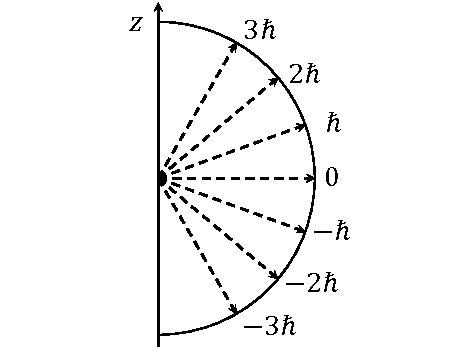
\includegraphics[width=0.7\textwidth,height=\textheight,keepaspectratio]{Seminar_06/pics/pic_01.pdf}
    \caption{Пример возможных значений проекции момента импульса на ось $z$.}
    \label{fig:sem_06_momet_projection}
\end{figure}

Теперь давайте посчитаем среднее значение квадрата этой проекции и среднее значение квадрата всего момента импульса (просто умножив первое выражение на 3 из-за изотропности по 3 осям):
\begin{gather*}
    \langle \hat{L_z^2}\rangle=\hbar^2\dfrac{l^2+ (l-1)^2 +\dots +(-l+1)^2 +(-l)^2}{2l+1} =\hbar^2\dfrac{\sum\limits_{m=-l}^{l}m^2}{2l+1} = \dfrac{\hbar^2}{3}l(l+1)\\
    \langle \hat{L^2}\rangle = \hbar^2l(l+1)
\end{gather*}

Так мы видим, что квадрат момента импульса тоже может быть только целым, но не равным квадрату в его проекции. Так же можно честно записать значение оператора квадрата момента импульса в сферических координатах и решить задачу на его собственные значения (они совпадают с решением выше) и собственные функции, но это существенно более сложная математики и строго рассматривается в курсе теоретической физики. Здесь я просто приведу пару формул. 
\begin{gather*}
     \hat{L^2} = -\hbar^2 \left[ \dfrac{1}{\sin{\theta}}\dfrac{\partial}{\partial\theta} \left(\sin{\theta}\dfrac{\partial}{\partial \theta}\right) + \dfrac{1}{\sin^2{\theta}}\dfrac{\partial^2}{\partial \varphi^2}\right]\\
     \hat{L^2} \psi = \langle \hat{L^2}\rangle \psi\\
     \psi = Y_{lm}(\theta; \varphi)
\end{gather*}

Здесь $Y_{lm}; n,m \in \{\mathbb{N}, 0\}$ --- специальные комплекснозначные сферические функции, которые можно посмотреть, например, в Ладавшице или Википедии.

Последнее, о чем стоит сказать в этой части, это приложение всей теории к <<квантовому ротатору>>. По сути, квантовый ротатор, это не что иное, как обычная молекула, момент инерции $I$ которой вдоль выбранной оси достаточно большой (много больше момента инерции атома). Вся теория для него верна, и его характерные уровни энергии это:
\begin{equation}
    E_l=\dfrac{\hbar^2l(l+1)}{2I}, l\in \mathbb{N}
\end{equation}

\subsection{Теория Бора для атома водорода}
Для начала отдадим дань теории, придуманной Нильсом Бором, для того чтобы описать поведение электрона в атоме водорода. Её основные постулаты это:
\begin{itemize}
    \item Наличие в атоме стационарных орбит, на которых электроны живут сколь угодно долго
    \item Излучение происходит только при переходе с одной орбиты на другую
    \item Момент импульса электрона квантуется
\end{itemize}

Далее у нас получается записать второй закон Ньютона (для электрона в атоме с зарядом $Z$) и последний постулат и решить систему:
\begin{gather*}
    \begin{cases}
     mvr = \hbar n; n\in \mathbb{N}\\[10pt]
     m\dfrac{v^2}{r} = \dfrac{Ze^2}{r}
     \end{cases}
     \Rightarrow
     \begin{cases}
     r_n = \dfrac{\hbar^2}{Ze^2m}n^2\\[10pt]
     E_n = -\dfrac{Z^2me^4}{2\hbar^2} \dfrac{1}{n^2} = -Z^2 Ry\dfrac{1}{n^2}
     \end{cases}
\end{gather*}
$Ry = 13.6$ эВ --- постоянная Ридберга, которая по физическому смыслу соответствует энергии ионизации атома водорода из основного состояния.

\begin{figure}[h]
    \centering
    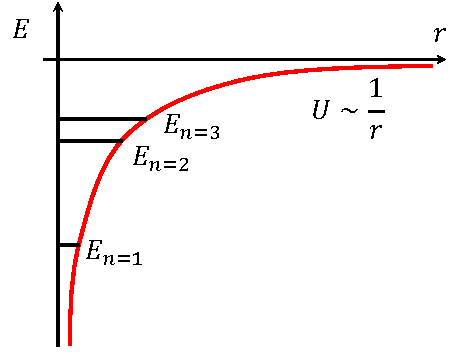
\includegraphics[width=0.6\textwidth,height=\textheight,keepaspectratio]{Seminar_06/pics/pic_02.pdf}
    \caption{Структура энергетических уровней в атоме водорода}
    \label{fig:sem_04_H_energy_levels}
\end{figure}

В целом мы видим, что теория достаточно строгая, все хорошо описывает, а если проверить спектр атома водорода, то и вообще совпадает с экспериментом. Однако это не совсем так. Для основного состояния электрона в атоме водорода полный момент импульса не равен 0, но это не так в реальной жизни. Поэтому вся эта теория не верна, а нужна нам для общего развития и конкретных оценок в задании. Как это можно проверить, мы обсудим на следующем семинаре. 

\subsection{Строгая теория для атома водорода}
Начнем с того, что мы не будем сильно углубляться в математику, оставив это теорфизикам, а больше сориентируемся на следствиях из теории. Начнем с того, что для атома водорода можно записать уравнение Шредингера в сферических координатах. 
\begin{gather}
\label{eq:sem_06_schrodinger_atom}
    -\dfrac{\hbar^2}{2m}\Delta\psi + U(r)\psi = E\psi\\
    -\dfrac{\hbar^2}{2m}\dfrac{1}{r^2}\dfrac{\partial}{\partial r}\left( r^2 \dfrac{\partial\psi}{\partial t}\right) + U(r)\psi +\dfrac{1}{2mr^2}\hat{L^2}\psi = E\psi
\end{gather}
Тут нужно отметить, что при записи Лапласиана переменные $\{r\}$ и $\{\theta; \varphi\}$ разделяются, при этом решение для угловой части мы уже записывали, и нам останется найти решение только для радиальной составляющей и перемножить их. Традиционно решение ищут в виде:
\begin{equation*}
    \psi(r, \theta, \varphi) = \dfrac{\xi(r)}{r}\times Y_{lm}(\theta; \varphi)
\end{equation*}

В результате у нас получается одномерная задача на функцию $\xi(r)$. Строгое решение я здесь не привожу, а когда нам понадобятся волновые функции в явном виде --- запишу ответ.
Первое, запишем финальный вид решения и обсудим следствия из него:
\begin{equation*}
    \psi_{nlm}(r, \theta, \varphi) = A \exp{(-\varkappa_n r)}r^l\left[\sum\limits_{i=0}^{n-l-1}a_{l+1+i}r^i\right]Y_{lm}(\theta, \varphi)
\end{equation*}
Здесь $A, \varkappa_n, a_n$ --- некоторые постоянные, которые нам не важны. Основной результат, получающийся из этого решения, следующий: у нас появилось 3 числа $l,m,n$, которые имеют вполне понятный смысл и интерпретацию. Подробнее про каждое из них:
\begin{itemize}
    \item $n = 1, 2, 3, \dots $ --- главное квантовое число. Отвечает за основной уровень энергии: чем больше, тем ближе энергия электрона к 0.
    \item $l = 0, 1, 2, \dots, n-1$ --- орбитальное квантовое число. Отвечает за полный момент импульса электрона для соответствующего уровня энергии $n$. Всегда меньше главного квантового числа. Исторически также принято обозначать буквами $\{s,p,d,f, \dots \} \sim \{0,1,2,3, \dots\}$.
    \item $m = -l, -l+1, \dots, l-1, l$ --- магнитное квантовое число, показывает проекцию полного момента на выделенную ось.
\end{itemize}

Если же построить плотность вероятности нахождения электрона ($\psi^2_{nlm}(r, \theta, \varphi)$), то можно получить явно те самые орбитали, про которые говорят химики.
\begin{figure}[h]
    \centering
    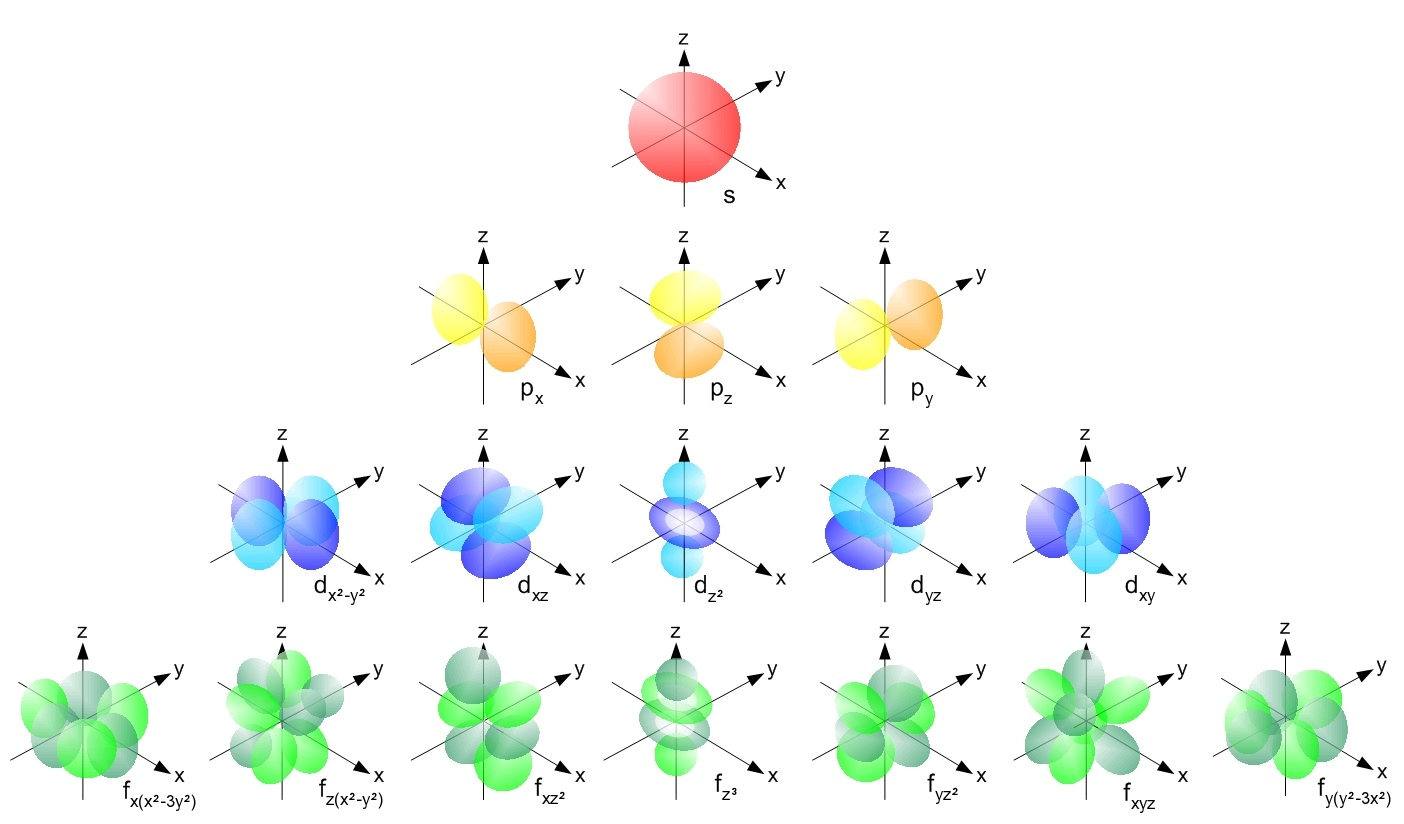
\includegraphics[width=\textwidth,height=\textheight,keepaspectratio]{Seminar_06/pics/Pic_03.jpg}
    \caption{Плотность вероятности электрона в водородоподобном атоме для различных значений квантовых чисел}
    \label{fig:sem_04_H_energy_levels}
\end{figure}
Уровни энергии в атоме также получаются из решения уравнения Шредингера \ref{eq:sem_06_schrodinger_atom} и совпадает с боровской теорией:
\begin{equation}
   E_n = -\dfrac{Z^2me^4}{2\hbar^2} \dfrac{1}{n^2} = -Z^2 Ry\dfrac{1}{n^2}
\end{equation}
А переходы между уровнями соответствуют испусканию или поглощению света. Обычно, когда говорят о постоянной Ридберга, имеют в виду постоянную, вычисленную при неподвижном ядре. При учёте движения ядра масса электрона заменяется приведённой массой электрона и ядра ($\mu = \frac{m_1 m_2}{m_1+m_2}$), и тогда
\begin{equation*}
    R=\dfrac{Ry}{1+m/M_{\text{яд}}}
\end{equation*}

Это может понадобиться в задачах на изотопический сдвиг (когда мы рассматриваем не водород, а дейтерий с массой ядра в 2 раза большей) или в экзотических случаях типа протон-антипротон (как раз такой есть в задании).


Последнее, о чем стоит сказать, это кратности вырождения состояний для разных $n$ --- то есть сколько всего <<вакансий>> у нас есть на соответствующем уровне. Для этого заполним таблицу:
\begin{table}[H]
\centering
\begin{tabular}{|l|l|l|l|l|l|}
\hline
\multicolumn{1}{|c|}{$n$} & \multicolumn{1}{c|}{$l$}                            & \multicolumn{1}{c|}{$m$}                                                                                            & \multicolumn{1}{c|}{Состояние}                       & \multicolumn{1}{c|}{Кратность вырождения}         & \multicolumn{1}{c|}{Всего состояний} \\ \hline
1                       & 0                                                 & 0                                                                                                                 & 1S                                                   & 1                                                 & 1                                    \\ \hline
2                       & \begin{tabular}[c]{@{}l@{}}0 \\ 1\end{tabular}    & \begin{tabular}[c]{@{}l@{}}0\\ 0, $\pm$ 1\end{tabular}                                               & \begin{tabular}[c]{@{}l@{}}2S\\ 2P\end{tabular}      & \begin{tabular}[c]{@{}l@{}}1\\ 3\end{tabular}     & 4                                    \\ \hline
3                       & \begin{tabular}[c]{@{}l@{}}0\\ 1\\ 2\end{tabular} & \begin{tabular}[c]{@{}l@{}}0\\ 0,$\pm$ 1\\ 0,$\pm$ 1, $\pm$ 2\end{tabular} & \begin{tabular}[c]{@{}l@{}}3S\\ 3P\\ 3D\end{tabular} & \begin{tabular}[c]{@{}l@{}}1\\ 3\\ 5\end{tabular} & 9                                    \\ \hline
\end{tabular}
\end{table}
Видно, что кратность вырождения квадратично растет с уровнем. На самом деле, в следующем семинаре мы узнаем, что она растет как $2n^2$: эта двойка появляется из-за спина.

\section{Практическая часть}
\subsection{Задача 4.7}
\label{task_4.7}
\paragraph{Условие} Найти среднее расстояние электрона от ядра в 1s-состоянии в атоме водорода. Волновая функция основного состояния $\psi_{100}(r, \theta, \varphi) = \dfrac{1}{\sqrt{\pi r_1^3}}\exp{\left(-\dfrac{r}{r_1} \right)}$, $r_1$ --- радиус первой Боровской орбиты.
\paragraph{Решение}
Эта задача является, по сути, отсылкой к прошлому семинару. Тут нам дана волновая функция, и надо найти среднее значение оператора координаты, проинтегрировав во всему пространству с учетом сферической симметрии:
\begin{equation}
    \langle r\rangle = \int\limits_0^{\infty} \psi^*_{100} r \psi_{100} 4\pi r^2 dr =\dfrac{1}{\pi r_1^3}\int\limits_0^{\infty} \exp{\left(- \dfrac{2r}{r_1} \right)} r^3 dr = \dfrac{3}{2}r_1
\end{equation}

\subsection{Задача 4.29}
\label{task_4.29}
\paragraph{Условие} В 1989 году в ЦЕРНе при пропускании медленных антипротонов через водородную камеру наблюдалось образование протонимума --- атома, состоящего из протона и антипротона. Энергия излучения, соответствующая переходу протониума из состояния 2p в состояние 1s оказалась равной 10,1 кэВ. Определить вклад сильного взаимодействия в разность энергии указанных уровней.
\paragraph{Решение}
Пока в задаче мало что понятно. Давайте её постепенно раскручивать и разбираться в условии. Первое, если у нас есть конструкция протон-антипротон, то это по своей сути тот же атом водорода, только массы положительной и отрицательной частиц равны между собой. Прекрасно, мы можем записать его урони энергии, ведь в теоретической части мы как раз отмечали, как меняется постоянная Ридберга, если учесть движение ядра:
\begin{equation*}
    E_n = - \dfrac{Ry}{1+m_e/m_p}\dfrac{1}{n^2} = -Ry\dfrac{m_p}{2m_e} \dfrac{1}{n^2} = -\dfrac{12.5}{n^2} \text{ кэВ}
\end{equation*}

Теперь надо разобраться с переходом между 2p и 1s состояниями. Здесь мы просто смотрим на цифру в начале описания состояния --- она будет отвечать за главное квантовое число и, соответственно, за уровень энергии. То есть, наблюдается переход с $n=2$ на $n=1$
\begin{equation*}
    \Delta E = 12.5\left(\dfrac{1}{1^2} - \dfrac{1}{2^2}\right) = 9.4 \text{ кэВ}
\end{equation*}

Полученный результат не совпадает с экспериментальным из-за того, что в наших расчетах мы использовали только потенциал кулоновского взаимодействия, но ведь есть еще и другие взаимодействия, которые могут оказаться существенными. Величина этого несовпадения $\delta E = 10.1 - 9.4 = 0.7$ кэВ. Именно это и есть вклад сильного взаимодействия. 


\subsection{Задача 5.11}
\label{task_5.11}
\paragraph{Условие} В опытах с равными молекулами измерялись энергии перехода между тремя последовательными уровнями энергии вращательной полосы двухатомной молекулы. Найти
квантовые числа $l$ этих уровней и момент инерции $I$ молекулы в этих случаях.
\begin{figure}[h]
    \centering
    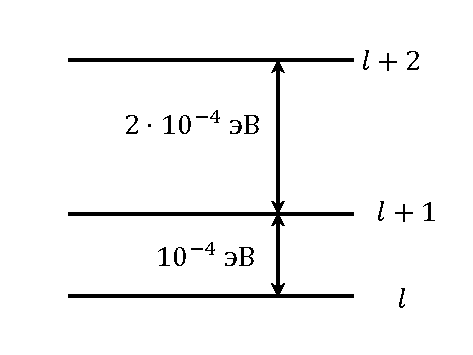
\includegraphics[width=0.5\textwidth,height=\textheight,keepaspectratio]{Seminar_06/pics/pic_04.pdf}
    \caption{ структура уровней энергии к задаче 5.11}
\end{figure}
\paragraph{Решение}
Поскольку уровни энергии последовательны, они соответствуют уровням с номерами $l, l+1, l+2$, а тогда сама энергия будет пропорциональна $l(l+1), (l+1)(l+2), (l+2)(l+3)$. Из соотношения энергии между уровнями найдем $l$:
\begin{equation*}
    \dfrac{2}{1} = \dfrac{(l+2)(l+3)-(l+1)(l+2)}{(l+1)(l+2)-l(l+1)} = \dfrac{l+2}{l+1} \Rightarrow l=0
\end{equation*}
Для нахождения момента инерции воспользуемся данными о переходе с $l=0$ на $l=1$:
\begin{gather*}
    \Delta E_{0\rightarrow 1} = \dfrac{\hbar^2 l(l+1)}{2I}\\
    I = \dfrac{\hbar^2}{\Delta E_{0\rightarrow 1}} = 6.9\cdot 10^{-39} \text{ г}\cdot\text{см}^2
\end{gather*}

\subsection{Задача 5.13}
\label{task_5.13}
\paragraph{Условие} Какова максимальная длина волны СВЧ-излучения, с помощью которой можно вызвать переход между ротационными уровнями молекул хлорa? Расстояние между ядрами атомов в молекуле $\text{Cl}_2$ равно $d = 2 \cdot 10^{-8}$ см. Относительная атомная масса изотопа хлора $A=35$.
\paragraph{Решение}
Максимальная длина волны соответствует минимальной частоте и, как следствие, минимальной энергии перехода. А она будет как раз между 0 и 1 уровнями (мы увидели это в предыдущей задаче). Осталось вспомнить как посчитать момент инерции, чтобы подставить его в формулу для энергии. Для двухатомных молекул все просто: $I = \mu d^2$, где $\mu$ --- приведенная масса этой молекулы. В нашем случае она равна $m_{\text{Cl}}/2 = 35/2 \cdot 1.6 \cdot 10^{-24}$ г, так как атомы в молекуле одинаковые. Теперь выразим максимальную длину волны из формулы для энергии:
\begin{equation*}
    \lambda = \dfrac{2\pi \hbar с m_{\text{Cl}} d^2}{2\hbar^2} = 2.1 \text{ см}
\end{equation*}


\subsection{Задача 5.25}
\label{task_5.25}
\paragraph{Условие} В угарном газе из-за возбуждения колебаний молекул наблюдается  пик поглощения инфракрасного излучения на длине волны $\lambda = 4,61$ мкм. Оценить амплитуду нулевых колебаний в молекуле угарного газа. Оценить температуру, при которой амплитуда тепловых колебаний превзойдет ее.
\paragraph{Решение}
Эта задача на квантовый гармонический осциллятор, про который мы говорили в прошлый раз. Мы помним, что энергия у его не бывает равна нулю из-за соотношения неопределнностей, и такая молекула колеблется с известной нам энергией $\hbar \omega/2$. Тогда мы можем записать эту энергию через коэффициент жесткости и амплитуду нулевых колебаний, а коэффициент жесткости выразить через частоту и приведенную массу:
\begin{gather*}
    \begin{cases}
       \dfrac{\hbar \omega}{2} = \dfrac{kA_0^2}{2}\\
       \omega^2 = \dfrac{k}{\mu}
    \end{cases} \Rightarrow \;\; A_0 = \sqrt{\dfrac{\hbar}{\mu \omega}} = 4,74\cdot 10^{-10} \text{ см}
\end{gather*}
Условие на температуру получается из сравнения энергии нулевых колебаний и характерной тепловой энергии:
\begin{equation*}
    kT = \dfrac{\hbar \omega}{2} \Rightarrow T\sim 3100 \text{ К}
\end{equation*}


\subsection{Комментарии к задачам из задания}
\paragraph{Нулевки} 
\paragraph{Задача 4.29} Решена, см. \ref{task_4.29}.
\paragraph{Задача 4.38} Задача на закон Мозли и экранирование, решена в задачнике.
\paragraph{Задача 4.42} Очень похожа на 4.41, решенную в задачнике.
\paragraph{Задача 4.45} Оценить радиус орбиты мюона и подумать, как это может повлиять на решение. 
\paragraph{Задача 5.16} Задача, почти что обратная к 5.13.
\paragraph{Задача 5.25} Решена, см. \ref{task_5.25}.
\paragraph{Задача 5.51} Для разных изотопов будет немного разная приведенная масса и, соответственно, момент инерции. Далее стандартные уровни энергии для ротатора.
\paragraph{Задача 5.55} Дублирую указание из учебника. Энергия, как функция уровня, должна расти монотонно. 

\end{document}
